%%This is a very basic article template.
%%There is just one section and two subsections.

%%******************************************************************************
%% FRONT PAGE
%%******************************************************************************

% \thispagestyle{empty}
% 
% %% Restart page counter.
% \setpagecounter{0}
% 
% %% Disable page anchor to avoid multiple page number definition warnings.
% \hypersetup{pageanchor=false}
% 
% \vspace{4cm}
% 
%  \textcolor{gray}{Execução:} \

%%==============================================================================




%\documentclass[a4paper,11pt,oneside,openany,brazilian,
%version=last,draft=false,]{report}

\documentclass[a4paper,11pt,oneside,openany,brazilian,version=last,draft=false,]{main}


%%******************************************************************************
%% DOCUMENT STYLE
%%******************************************************************************


% \usepackage{graphicx}      % include this line if your document contains figures
% \usepackage{natbib}        % required for bibliography
% \usepackage{enumerate}
% \usepackage[utf8]{inputenc}
% \usepackage{graphicx}
% \usepackage{float}
\usepackage[centerlast,small,sc]{caption}
\setlength{\captionmargin}{30pt}
% \usepackage[brazilian]{babel}
% \usepackage[none]{hyphenat}
% \sloppy


\usepackage{graphicx}
\usepackage{natbib}        % required for bibliography
\usepackage[utf8]{inputenc}
\usepackage{mybook}
\usepackage{float}
\usepackage{fancyhdr}
\usepackage{pdfpages}
\usepackage {subcaption}
\usepackage{color}
\sloppy  


\pdfcompresslevel = 9
\oddsidemargin = 31pt
\topmargin = 20pt
\headheight = 12pt
\headsep = 25pt
\textheight = 592pt
\textwidth = 390pt
\marginparsep = 10pt
\marginparwidth = 35pt
\footskip = 30pt

\usepackage[top=1.5in, bottom=1.25in, left=0.8in, right=0.8in]{geometry}




\begin{document}



%%******************************************************************************
%%
%% frontpage.tex
%%
%%******************************************************************************
%%
%% Title......: ROSA - Stoplog Inspection
%%
%% Author.....: GSCAR-DFKI
%%
%% Started....: Nov 2013
%%
%% Emails.....: renan028@gmail.com
%%
%% Address....: Universidade Federal do Rio de Janeiro
%%              Caixa Postal 68.504, CEP: 21.945-970
%%              Rio de Janeiro, RJ - Brasil.
%%
%%******************************************************************************


%%******************************************************************************
%% FRONT PAGE
%%******************************************************************************




%%==============================================================================
%% FRONT PAGE CONTENTS
%%==============================================================================
\thispagestyle{empty}

%% Restart page counter.
\setpagecounter{0}

%% Disable page anchor to avoid multiple page number definition warnings.
\hypersetup{pageanchor=false}

\vspace{4cm}

 \textcolor{gray}{Execução:} \\
\\
\begin{minipage}{\textwidth}
	\centering
       
	
\includegraphics[width=0.3\textwidth]{logos/lead-logo}
	
\end{minipage}

\vspace{2cm}

\textcolor{gray}{Financiamento: } \\ 
\\
\begin{minipage}{\textwidth}
	\centering
	
	
\includegraphics[width=0.3\textwidth]{logos/esbr-logo}
	
\includegraphics[width=0.3\textwidth]{logos/aneel-logo}

	
\end{minipage}

\vspace{4cm}

\begin{table}[ht!]
	\centering
	\begin{tabular}{r l|l p{12cm} }
		\textcolor{gray}{Projeto} &&& \textbf{\Large EMMA}\\
			&&& \textbf{Robô para Inspeção de Turbinas}\\
			&&& \\
		\textcolor{gray}{Título} &&& \textbf{Relatório de Viagem}\\
		\textcolor{gray}{PD} &&& 6631-0003/2015 \\
		\textcolor{gray}{Contrato} &&& Jirau 09-15\\
		\textcolor{gray}{Coordenador} &&& Ramon Romankevicius Costa \\
		\textcolor{gray}{Gerente} &&& Breno Bellinati de Carvalho \\
		\textcolor{gray}{Período} &&& 01.03.2015 - 01.07.2016 \\
		\textcolor{gray}{Data:} &&& \today \\
	\end{tabular}
\end{table}


\cleardoublepage

%%==============================================================================
%% AUTHORS AND VERSION PAGE
%%==============================================================================
\begin{onecolumn}
\thispagestyle{empty}

%% Restart page counter.
\setpagecounter{0}

\begin{center}
  %% Version section. --------------------------------------------------------

  
 \vfill
  %% Project section. --------------------------------------------------------


  %% Authors section. --------------------------------------------------------

  \center{\LARGE Participante(s)}
  
  \vspace{0.50cm}



  \begin{center}
    \begin{tabular}{| l | l | l | l | l |}
    
    \hline
   	 Nome 					& Função			 & Qualificação 	& Instituição	 & CPF \\ \hline
   	 Ramon Romankevicius 		& Coordenador 	& DO			 & UFRJ 		& 310.036.646-87\\			\hline
%    	Alessandro Jacoud 			& Pesquisador 		& DO 			& UFRJ 	& 028.503.687-41\\ 			\hline
   	Julia Campana 			& Pesquisador		 & SU 			& UFRJ 	& 102.517.697-98\\ 			\hline
   	Renan Freitas 				& Pesquisador 		& SU 			& UFRJ 	& 129.325.817-24\\ 		
   	\hline Eduardo Elael 				& Pesquisador 		& SU 			& UFRJ	 & 045.287.677-08\\ 			\hline
  	Gabriel Alcantara 			& Pesquisador 		& SU 			& UFRJ 	& 136.759.937-79\\
  	\hline
%   	\hline André Figueiró 			& Pesquisador 		& SU 			& UFRJ 	& 124.207.057-050\\ 			\hline
   	Alana Monteiro 			 & Auxiliar Adm.	 & SU 			& UFRJ 	& 147.881.217-60\\ 		
   	\hline Patrick  Paranhos 			& Pesquisador 		& MS 			& CIR 	& 092.144.157-65\\ \hline
	Breno Carvalho				 & Gerente 		& SU 			& ESBR 	& 0000000\\ 	
\hline
	Gizelle Ferreira 			& Auxiliar Adm. 	& SU 			& ESBR 	& 0000000\\ 
\hline

    
    \hline 
    \end{tabular}
\end{center}

\end{center}
\end{onecolumn}

\newpage

%% Enable page anchor again.
\hypersetup{pageanchor=true}


\begin{twocolumn}
% \title{Relatório de Viagem}
% \author{Julia Campana, Eduardo Elael}
% \date{27/04/15 - 01/05/15}
% \maketitle


% \begin{flushright}
%   \emph{Versão:} 07/maio/2014
% \end{flushright}


\section{Introdução}
A viagem a Jirau realizada entre os dias 27 de Abril e 01 de Maio teve como
objetivo coletar informações para o a fase conceitual do Projeto EMMA. 

\section{Objetivo de Viagem}
\begin{itemize}
  \item Breve apresentação SOTA (Estado da Arte de sistema robóticos
  seme\-lhantes);
  \item Alinhamento técnica com Rijeza, perguntas e respostas relacionadas ao
  processo de hardcoating (descritas no artigo);
\item Definição das tarefas do robô EMMA com a ESBR;
\item Discussão do problema relacionadas ao ambiente da turbina (descritas no
artigo) 
\item Demonstração do processo de hardcoating pela Rijeza;
\item Visita à uma turbina para inspecionar os pontos de acesso.;
\end{itemize}


\section{Execução}
Em um primeiro momento foi realizada a reunião para a apresentação de estado da
arte de sistemas robóticos que executam tarefas semelhantes às que serão
realizadas, seguida de perguntas e respostas aos técnicos da Rijeza e ESBR para
esclarecimento dos aspectos técnicos pertinentes ao projeto.

\begin{figure}[H]
\centering
%\begin{subfigure}[b]{0.46\textwidth}
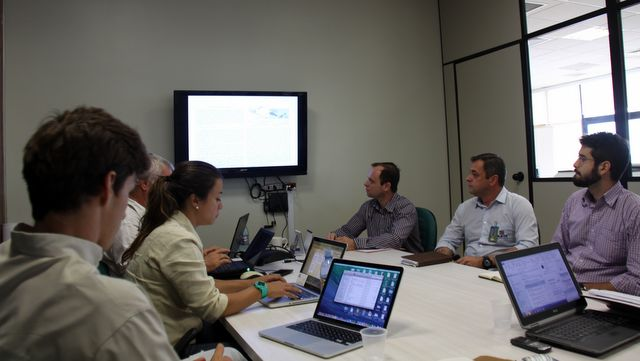
\includegraphics[width=\columnwidth]{Fotos/img_4836.jpg}
\caption{Reunião com Rijeza e ESBR.}
\label{fig:gull}
%\end{subfigure}%
%\quad
\end{figure}
\begin{figure}[H]
\centering
%\begin{subfigure}[b]{0.46\textwidth}
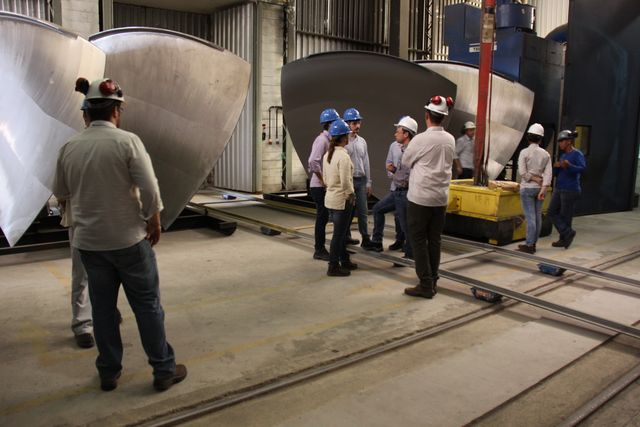
\includegraphics[width=\columnwidth]{Fotos/img_4881.jpg}
\caption{Equipe visita o galpão da Rijeza.}
\label{fig:tiger}
%\end{subfigure}
\end{figure}

% \begin{figure}[H]
% \centering
% 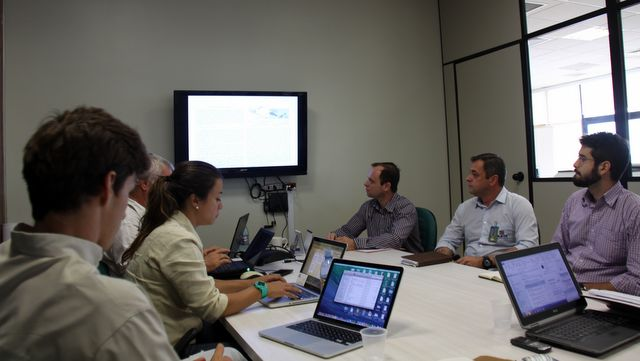
\includegraphics[width=0.85\textwidth]{Fotos/img_4836.jpg}
% \caption{Reunião com Rijeza e ESBR.}
% \end{figure}

Posteriormente, visitamos as instala\-ções da Rijeza dentro da usina para
presenciar o funcionamento do robô que executa o \textit{hardcoating}, assim como o
estado das pás onde o \textit{hardcoating} já havia sido aplicado. Visando compreender
melhor o processo de metalização, suas etapas e especificidades quando realizado
sobre uma pá da turbina.

\begin{figure}[H]
\centering
%\begin{subfigure}[b]{0.46\textwidth}
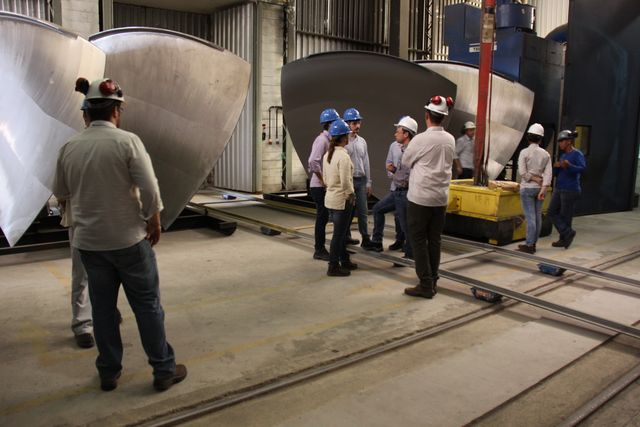
\includegraphics[width=\columnwidth]{Fotos/img_4881.jpg}
\caption{Equipe do projeto EMMA visita o galpão da Rijeza para verificar o
processo de inspeção vigente.}
\label{fig:gull}
%\end{subfigure}%
%\quad
\end{figure}
\begin{figure}[H]
\centering
%\begin{subfigure}[b]{0.46\textwidth}
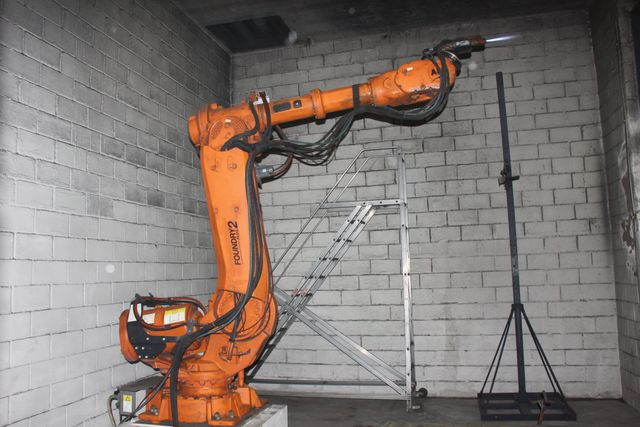
\includegraphics[width=\columnwidth]{Fotos/img_4858.jpg}
\caption{Instalações da Rijeza: Robô Industrial utilizado para aplicação de hardcoating.}
%\end{subfigure}
\end{figure}

% \begin{figure}[H]
% \centering
% 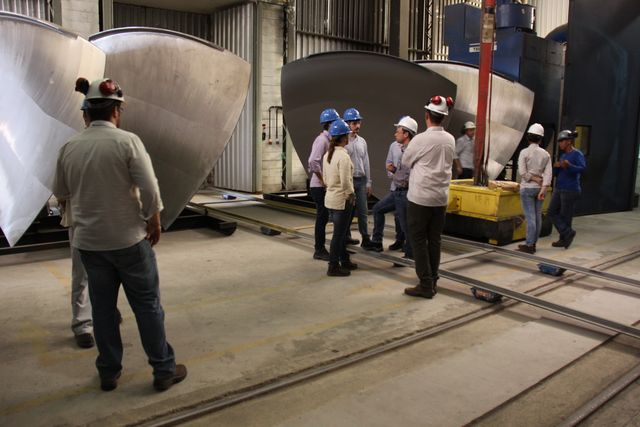
\includegraphics[width=0.85\textwidth]{Fotos/img_4881.jpg}
% \caption{Equipe visita o galpão da Rijeza.}
% \end{figure}
% 
% \begin{figure}[H]
% \centering
% 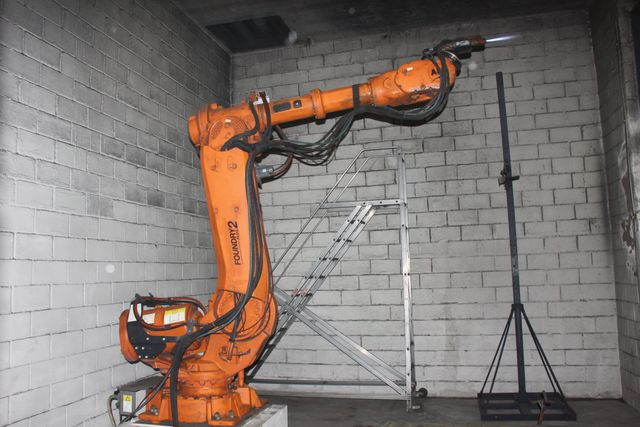
\includegraphics[width=0.85\textwidth]{Fotos/img_4858.jpg}
% \caption{Instalações da Rijeza: Robô Industrial utilizado para
% aplicação de hardcoating.}
% \end{figure}

% -----------------------------------------------------------------

\begin{figure}[H]
\centering
%\begin{subfigure}[b]{0.46\textwidth}
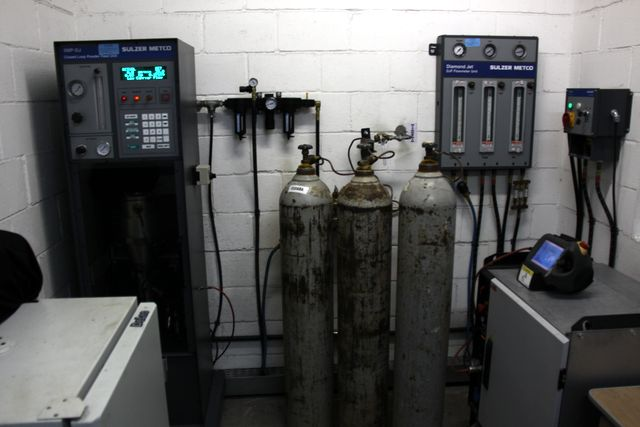
\includegraphics[width=\columnwidth]{Fotos/img_4850.jpg}
\caption{Instalações da Rijeza: secador, dosador, cilindros de gases, medidores,unidade de segurança e o console do robô.}
\label{fig:gull}
%\end{subfigure}%
%\quad
\end{figure}
\begin{figure}[H]
\centering
%\begin{subfigure}[b]{0.46\textwidth}
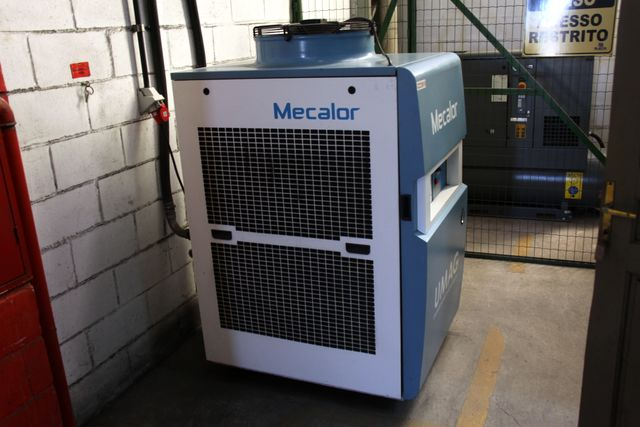
\includegraphics[width=\columnwidth]{Fotos/img_4852.jpg}
\caption{Instalações da Rijeza: Maquinário utilizado, equipamentos como cooler e
compressor ao fundo do galpão onde inspeção é realizada.}
%\end{subfigure}
\end{figure}

% \begin{figure}[H]
% \centering
% 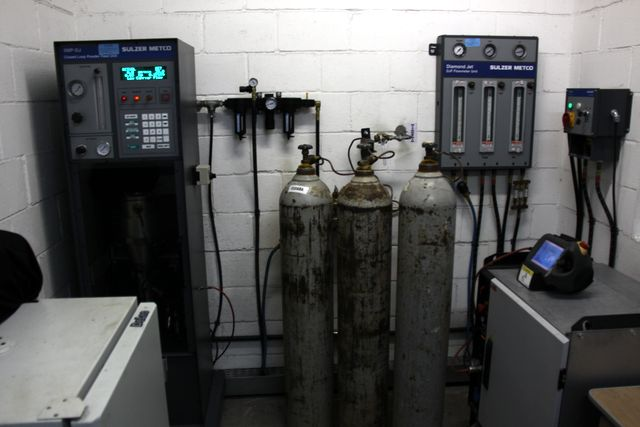
\includegraphics[width=0.85\textwidth]{Fotos/img_4850.jpg}
% \caption{Instalações da Rijeza: secador, dosador, cilindros de gases, medidores,
% unidade de segurança e o console do robô.}
% \end{figure}
% 
% \begin{figure}[H]
% \centering
% 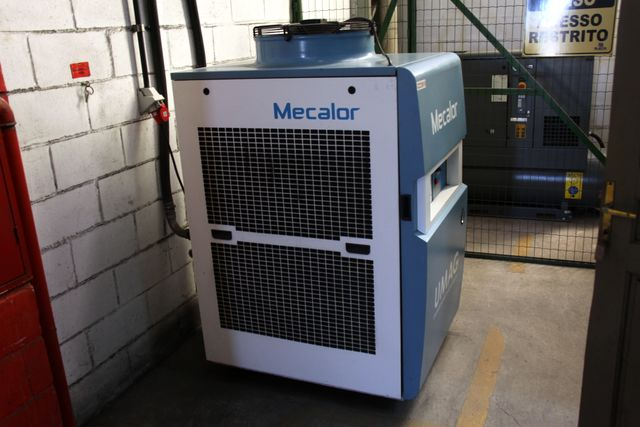
\includegraphics[width=0.85\textwidth]{Fotos/img_4852.jpg}
% \caption{Instalações da Rijeza: cooler e compressor ao fundo.}
% \end{figure}

% -----------------------------------------------------------------

Na parte da tarde visitamos uma unidade geradora para nos familiarizamos com o
local onde a aplicação de hardcoating será feita, nosso objetivo foi inspecionar
os locais de acesso, a montagem dos andaimes e a geometria da hélice.

% -----------------------------------------------------------------

\begin{figure}[H]
\centering
%\begin{subfigure}[b]{0.46\textwidth}
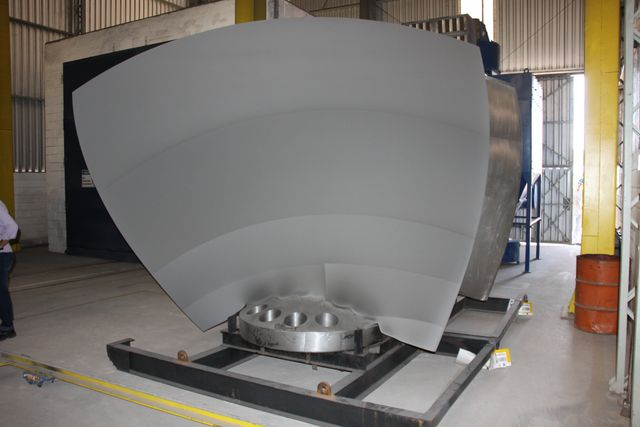
\includegraphics[width=\columnwidth]{Fotos/img_4886.jpg}
\caption{Pá já com Hardcoating aplicado.}
\label{fig:gull}
%\end{subfigure}%
%\quad
\end{figure}
\begin{figure}[H]
\centering
%\begin{subfigure}[b]{0.46\textwidth}
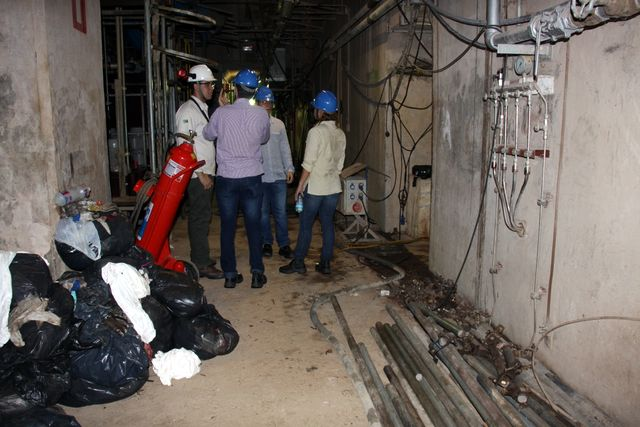
\includegraphics[width=\columnwidth]{Fotos/img_4905.jpg}
\caption{Acesso a unidade geradora.}
%\end{subfigure}
\end{figure}


% \begin{figure}[H]
% \centering
% 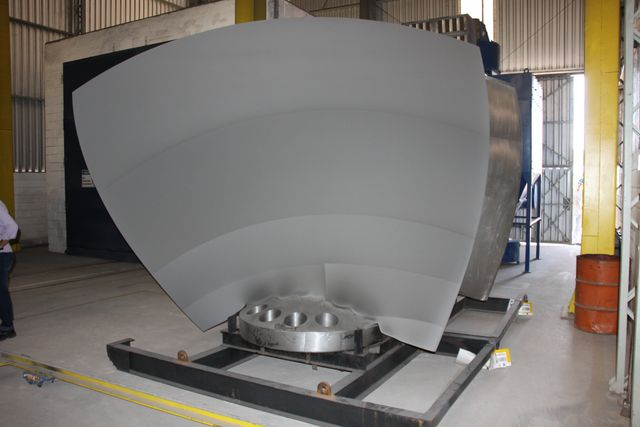
\includegraphics[width=0.85\textwidth]{Fotos/img_4886.jpg}
% \caption{Pá já com Hardcoating aplicado.}
% \end{figure}
% 
% \begin{figure}[H]
% \centering
% 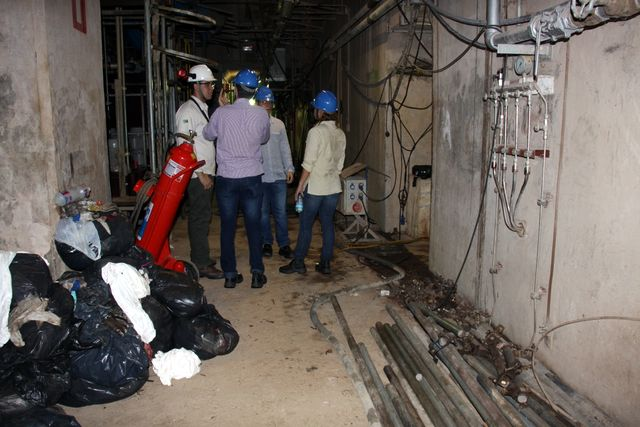
\includegraphics[width=0.85\textwidth]{Fotos/img_4905.jpg}
% \caption{Corredor de acesso unidade geradora.}
% \end{figure}

% -----------------------------------------------------------------






\begin{figure}[H]
\centering
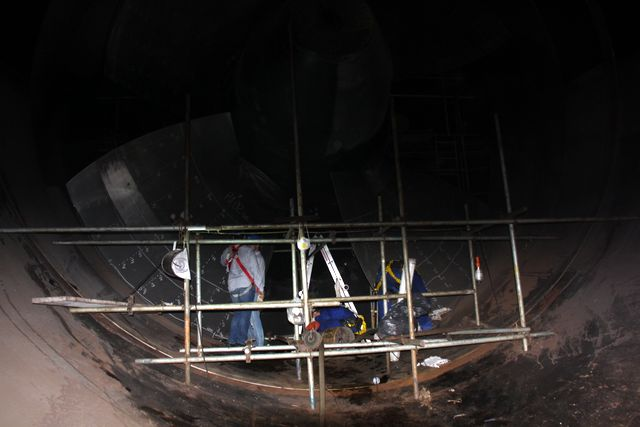
\includegraphics[width=\columnwidth]{Fotos/img_4931.jpg}
\caption{Montagem de andaimes dentro da unidade geradora.}
\end{figure}

\begin{figure}[H]
\centering
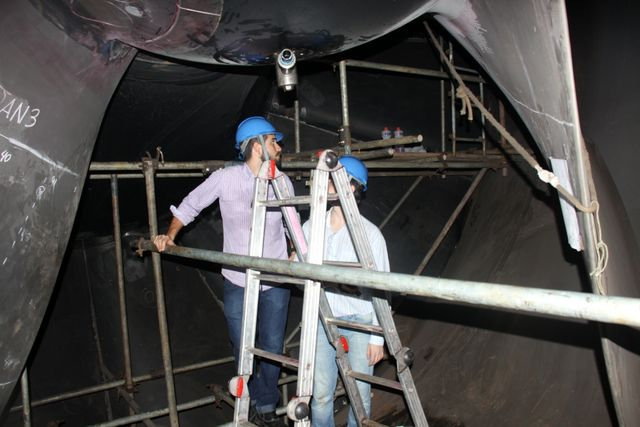
\includegraphics[width=\columnwidth]{Fotos/img_4966.jpg}
\caption{Engenheiros medem hélices.}
\end{figure}

% -----------------------------------------------------------------
\begin{figure}[H]
\centering
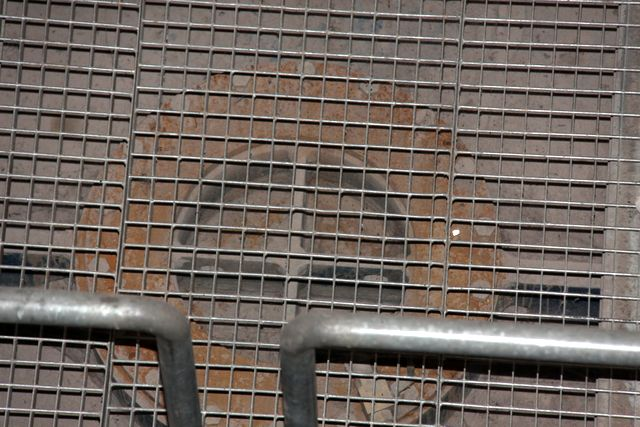
\includegraphics[width=\columnwidth]{Fotos/img_4978.jpg}
\caption{Em detalhe a escoltilha de acesso superior.}
\end{figure}

O segundo dia em Jirau foi voltado para a formulação dos conceitos possíveis
para o Robô EMMA. Em um primeiro momento avaliamos os braços mecânicos
disponíveis no mercado e todas suas possíveis aplicações no espaço da unidade
gerador onde a inspeção deve acontecer. Em seguida, levantamos hipóteses sobre
as possíveis vias de entradas e suas implicações. 

\section{Resultado}
A viagem se mostrou de grande relevância para a viabilidade técnica do projeto,
uma vez que nos deu parâmetros para formular os conceitos que serão explorados
como soluções para a inspeção de turbinas. Realizamos as reuniões
necessárias, a inspeção da unidade geradora, bem como conhecemos as instalações
da Rijeza onde o hardcoating é feita. No ultimo dia organizamos tais informações
para que sejam devidamente adicionas em nosso Relatório Técnico.
\end{twocolumn}
\end{document}
